Λόγω του μεγάλου αριθμού αριθμητικών παραμέτρων του μοντέλου, είναι απαραίτητη η ανάλυση
ευαισθησίας του μοντέλου σε αυτές τις παραμέτρους. Από την ανάλυση ευαισθησίας μπορεί κανείς
να αποφανθεί ποια μεγέθη χρήζουν πιο λεπτομερούς προσδιορισμού ή μέτρησης, αλλά και τον εντοπισμό
των κυρίαρχων παραμέτρων στη συμπεριφορά του μοντέλου. Για αυτή την ανάλυση, λοιπόν, επιλέχθηκε
να θεωρηθούν οι φυσικές παράμετροι ως σταθερές, καθώς αφενός αποτελούν φυσικά μεγέθη τα οποία
θα ήταν λάθος να μεταβάλλονται αυθαίρετα και αφετέρου είναι μεγέθη άμεσα μετρήσιμα με κατάλληλο
σχεδιασμό δοκιμών.\\[0.25cm]

Επιλέγονται, επομένως, προς ανάλυση οι παράμετροι του θερμοδυναμικού μοντέλου $p_{1\dots6}$, 
και ως αντικειμενικό μέγεθος σύγκρισης επιλέγεται η RMS θερμοκρασία πέλματος για έναν γύρο 
οχήματος Formula 1 στην πίστα \textit{Circuit de Barcelona-Catalunya}. Τα μεγέθη που περιγράφουν
το όχημα αλλά και η δομή του μοντέλου αναλύονται στα επόμενα κεφάλαια. Για την ποιοτική ανάλυση
ευαισθησίας επιλέχθηκε να απομονωθεί ενδεικτικά ο εμπρόσθιος αριστερός τροχός (FL).\\[0.5cm]

\noindent Στον πίνακα \ref{tab:params_thermal} φαίνονται τυπικές τιμές των παραμέτρων και σύντομη
επεξήγηση τους.

\begin{figure}[ht!]
    \begin{center}
        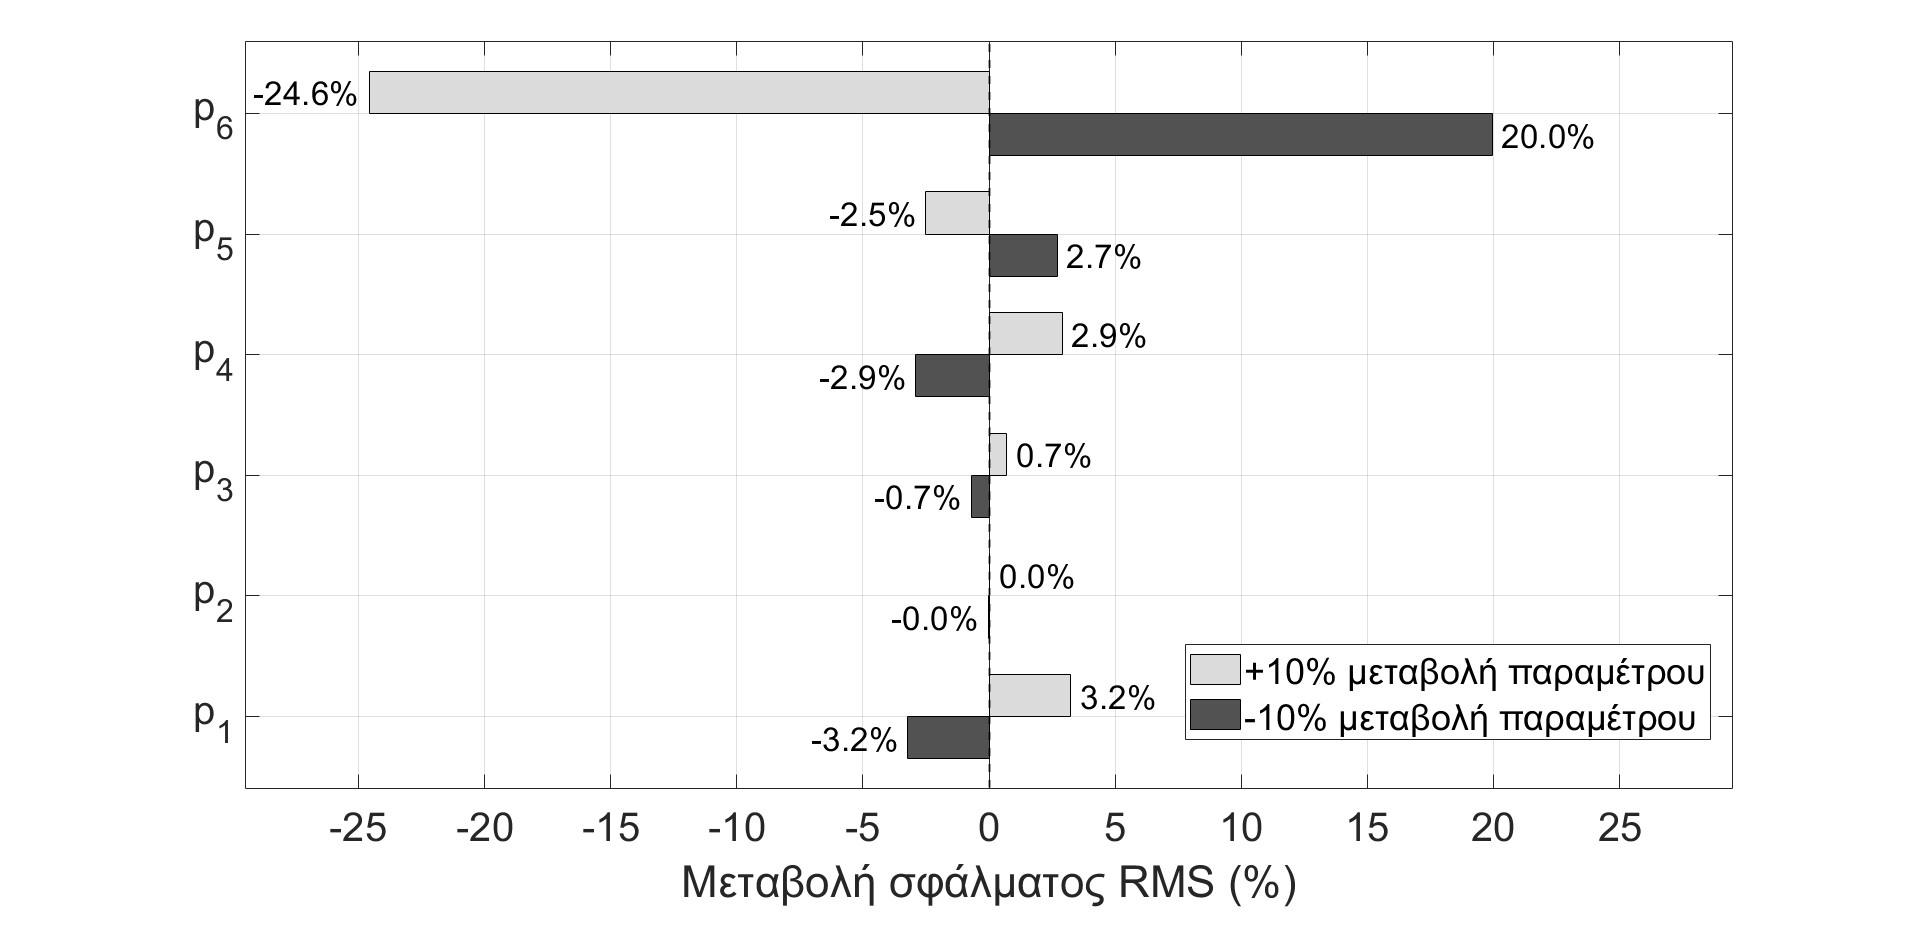
\includegraphics[width=\textwidth]{figures/sensitivity_analysis.jpg}
    \end{center}
    \caption{Ευαισθησία παραμέτρων θερμοδυναμικόυ μοντέλου -- μεταβολή RMS θερμοκρασίας}
   \label{fig:sensitivityAnalysis} 
\end{figure}

Από τα αποτελέσματα που φαίνονται στο \cref{fig:sensitivityAnalysis} παρατηρείται πως κυρίαρχος
παράγοντας είναι η παράμετρος $p_6$ (εκθέτης ταχύτητας στο μοντέλο ψύξης από συναγωγή). Αυτό το
αποτέλεσμα δεν προξενεί εντύπωση καθώς η συναγωγή είναι ο κύριος μηχανισμός ψύξης του ελαστικού
στις ευθείες, ενώ επιπλέον, τα αγωνιστικά οχήματα, όπως το όχημα της ανάλυσης, σημειώνουν πολύ
υψηλή ταχύτητα της οποίας τη συνεισφορά ενισχύει η παράμετρος $p_6$. Οι υπόλοιπες παράμετροι
σημειώνουν αναμενόμενες διαφορές στη μορφή τους, παρ'όλα αυτά φαίνεται να μην ενισχύουν σε 
τόσο μεγάλο βαθμό μικροδιαφορές στις εισόδους. Τέλος, αξίζει να παρατηρηθεί πως το μοντέλο
φαίνεται να "συγχωρεί" αρκετά στις τιμές των παραμέτρων $p_2,  p_3$, που ελέγχουν τη συνεισφορά
του έργου υστέρησης λόγω διαμήκους και εγκάρσιου φορτίου. Αυτό προκαλεί ιδιαίτερο ενδιαφέρον
καθώς υποδηλώνει πως στο έργο υστέρησης συνεισφέρει σχεδόν αποκλειστικά το κατακόρυφο φορτίο $F_z$
που έχει άλλωστε και το μεγαλύτερο μέτρο.\\[0.5cm]
